\chapter{塑闪阵列探测器的建造}
\label{ch:construction}
相比于地面使用,空间项目对探测器提出了具有更加苛刻的使用条件和更加严格的质量要求。
这不仅意味着要对探测器各部件进行特殊设计以适应火箭发射和空间使用环境,而且探测器的组件生产和整体装配必须遵循一定的建造规范并辅以严格的质量控制程序以保证其达到设计要求和质量。
塑闪阵列探测器的具体设计已经在第\ref{ch:description}章进行了梳理,本章将对它的实际建造过程进行简单介绍。

指导塑闪阵列探测器建造的有两条基本原则:一是要实现其功能要求,二是满足其质量要求。
PSD由探测器主体功能模块,高压扇出模块,前端电子学模块以及机械支撑模块这四部分组成。
其中,高压扇出模块、前端电子学模块和机械支撑模块都由专业的外包单位负责其建造和质量控制,实验室中我们只负责探测器主体功能模块中各探测单元的建造,主要包括是PMT组件以及塑闪单元条组件。
我们还在实验室中将上述四个模块组装成探测器整体,最终完成了塑闪阵列探测器的建造工作。

\section{PMT的筛选}
\label{sec:construction:pmt_selection}
PSD由82个探测单元模块组成,并要求它们之间的MIP能量响应一致性好于$\SI{25}{\percent}$。
PSD探测单元模块的能量响应是由R4443的Dy8增益以及塑闪单元条的衰减长度共同决定的。
光电倍增管具有较大的个体差异性,根据上一章\ref{sec:pmt_test:relative_gain}节的测试结果,不同R4443的Dy8增益最大可以相差一个量级;
而对于塑闪单元条来说,不同衰减长度导致的光输出差异最大不超过\SI{30}{\percent}(见\ref{sec:construction:bar_production}节的结果)。
因此,选择性能参数相近的R4443管子对保证探测单元模块的一致性尤为关键。
我们把PSD中PMT的筛选过程提取出来单独作为一节,对其进行详细描述。

首先,我们对所有待选的R4443管子进行了质量筛选,主要有:1)根据Hamamatsu提供的出厂测试参数淘汰阳极暗电流过大和工作状态稳定性(Drift,见\cite{hamamatsu})较差的管子;2)淘汰尺寸超过标准误差以及光阴极和外观有瑕疵的管子,由于PMT组件装配时对R4443的尺寸具有严格要求,因此我们在实验室对所有R4443裸管的尺寸进行了测量,另外我们还对管子的光阴极和玻璃管体表面进行了细致的检查以排查有细微裂纹的管子;3)淘汰参加了出厂前力学检测的管子,我们要求Hamamatsu随机抽取部分该批次的R4443管子进行振动和冲击测试,测试结果证明了R4443的力学性能够满足PSD的设计要求,但出于保守考虑,这些经历了力学测试的管子将不会安装到PSD探测器上。
这轮筛选中被淘汰的管子数量并不多,而且它们虽然不能够满足PSD的质量要求,但仍能在地面项目中继续使用。

之后,我们基于R4443的增益特性曲线与Dy58比值特性曲线,依照增益与动态范围两个方面的需求进行了一步的筛选,淘汰了具有极端特性的管子并确定了被选管子的工作电压档位。
第\ref{ch:pmt_test}章得到的Dy58比值特性曲线是绝对测量的结果,因此可以直接使用;
而得到的Dy8增益特性曲线是相对测量的结果(详见\ref{sec:pmt_test:relative_gain}节),不能直接使用。
为了在PSD的PMT筛选过程中使用该曲线,我们以某中一只管子的真实MIP响应为参照来计算其它所有管子的MIP响应,原理如下:
\begin{enumerate}
	\item 从待选管子中任选一支R4443,我们将其称为$PMT_{ref}$,$PMT_{ref}$与其它所有待选管子一样,在第\ref{ch:pmt_test}章中已经得到了它的增益特性曲线。
	\item 从待选的塑闪单元条中选取一根衰减长度在均值附近的条子,并将它与$PMT_{ref}$耦合成PSD的探测单元模块。该单元模块的另一端也耦合上PMT以保证其结构与实际情况完全一致,并且模块的装配和使用的材料也与实际使用的完全一致。
	\item 使用宇宙线对该单元模块中心位置处的MIP响应进行测试,考察$PMT_{ref}$对MIP入射光强$L_{mip}$的响应。通过调节$PMT_{ref}$的电压,我们将它的MIP响应中心值移到到设计值附近,令这个值为$A_{mip}$。这个工作电压就是$PMT_{ref}$的最佳工作电压,而此时的$PMT_{ref}$增益就是我们的参考增益,我们期望其它管子也工作在这个增益下。
	\item 为方便计算,我们没有使用以$G_{relative}$表述的相对增益测试结果,而是直接使用了以$A_{corr}$表述的结果,即增益特性曲线中没有消去入射光强量(详见\ref{sec:pmt_test:relative_gain}节)。我们选取了最弱入射光强(令其强度为$L_{test}$)测得的Dy8增益特性曲线,并计算出最佳工作电压下$PMT_{ref}$对该光强的响应中心值为$A_{test}$。
	\item $A_{test}$与MIP响应最佳值的比值,就是测试用的入射光强与实际的MIP入射光强的比值,即
	\begin{equation}
		\frac{A_{mip}}{A_{test}} = \frac{L_{mip}}{L_{test}}
		\label{eq:construction:pmt_selection}
	\end{equation}
	由上式可以推得$A_{mip}=A_{test}L_{mip}/L_{test}$,这意味着:如果其它管子在$L_{test}$入射光强下的响应中心值也为$A_{test}$,则它们耦合到塑闪单元条上后对MIP的响应中心值就是我们期望的设计值$A_{mip}$,而此时的增益就是最佳增益。
	由于我们已经得到了所有管子在$L_{test}$入射光强下的增益特性曲线,因此可以根据$A_{test}$值反推出各个管子的最佳工作电压。
\end{enumerate}
实际筛选中,$A_{mip}$被确定为450道,而我们选择的参考PMT所对应的$A_{test}$值在700道左右。

DAMPE高压单机只能提供不连续的高压档位且档位间隔为\SI{30}{V},而PSD只有7个工作电压档位可以使用(见\ref{sec:description:psd_hv}节)。
这极大限制了PSD的PMT筛选,我们只能尽量选择这样一些管子,使得它们的额定工作电压档位与最佳工作电压值尽量接近。
为了保留档位调节的余地,我们以\SI{810}{V}、\SI{840}{V}、\SI{870}{V}和\SI{900}{V}这四个档位为额定工作电压档,具体的筛选流程如下:
\begin{enumerate}
	\item 淘汰具有极端增益的管子。根据最小入射光强得到的Dy8增益特性曲线,计算每个管子对应于$A_{test}$时的工作电压,淘汰最佳工作电压在$\SI{790}{V}\sim\SI{900}{V}$范围外的管子。
	\item 确定额定工作电压。根据最小入射光强得到的Dy8增益特性曲线,分别计算SI{810}{V}、\SI{840}{V}、\SI{870}{V}和\SI{900}{V}四个电压档位下的响应中心值$A_{real}$,淘汰所有四个$A_{real}$值都在区间$[A_{test}-100,A_{test}+100]$范围外的管子。如果只有一个电压档位下的$A_{real}$值在该区间内,则这个档位就是该PMT的额定工作电压档位;如果多个电压档位下的$A_{real}$值在该区间内,则该PMT的额定电压由后面的筛选步骤确定。大部分管子在这一步就确定了额定工作电压档位。
	\item 淘汰动态范围不合适的管子。根据下面的公式可以计算出额定工作电压下各管子的动态范围上限$D_{range}$:
	\begin{equation}
		D_{range} = 12000\cdot G_{58} / (A_{mip}\cdot \frac{A_{real}}{A_{test}})
		\label{eq:construction:dynamic_range}
	\end{equation}
	其中,$12000$是Dy5通道的有效线性范围,$G_{58}$是根据Dy58比值增益曲线计算出的该管子在额定工作电压下的Dy58比值,而其它符号的定义同之前的定义一样。
	我们淘汰了$D_{range}$在区间$[1200,1400]$范围外的管子。
	\item 淘汰Dy8增益随电压变化异常的管子。DAMPE设计寿命为3年。由于寿命的原因,在DAMPE运行后期,PSD塑闪单元条的光产额和光电倍增管的增益都有可能减小,此时需要提高R4443的工作档位以保持PSD的探测性能不发生重大变化。因此,我们计算了提高三个档位后,即在额定工作电压值上再加90V后,R4443的Dy8增益相对于原来的比值,并淘汰了计算结果在区间$[1.6,2]$范围外的管子。这样就能保证提高工作电压档位后,PSD各探测单元模块间的一致性也会不发生巨大变化。
\end{enumerate}

经过上述两轮筛选过程,我们最终从570支R4443裸管中挑选出了190支管子,并确定了它们的额定工作电压档位。
这些管子将会经历完整的PMT组件生产流程(详见\ref{sec:construction:pmt_procedure}节),其中的164支最终会被安装到PSD探测器上,额外的26支管子将作为备份,以防组件生产过程出现的意外情况(如PMT损伤,PMT组件质量不合格等等)。

\section{PMT组件的生产}
\label{sec:construction:pmt_production}

\subsection{结构简介}
\label{sec:construction:pmt_assembly}
一个完整的PMT组件包括:R4443裸管,Base电路板,EJ-560硅脂垫片,PMT的铝合金保护套,高压和信号线缆。
为了更好地保护PMT组件,我们把R4443裸管、Base电路板以及硅脂垫片这三部分封装在一个硅胶保护套中,以减弱火箭发射时产生的剧烈振动和冲击对各部件的影响。
硅胶保护套可以分为两段,分别由不同的材料组成:
\begin{itemize}
	\item 避光部分。PMT是光敏器件,虽然PSD的机械结构设计是密封不透光的,为了以防万一,我们还是给光电倍增管设计了专门的避光措施。这部分胶体覆盖整个R4443裸管和硅脂垫片,并将它们连为一体。它由黑色材料构成,可以有效屏蔽外界光干扰。
	\item 绝缘部分。PSD分压器在工作时需要加载近千伏的高压,而太空中空气密度极低,再加上Base电路板的设计紧凑,板上各元器件间的距离较近,这些都大大增加了高压打火的概率。这部分胶体与前面的避光胶体部分紧密粘连,并完满填充了Base电路板上元器件间的空间。它由绝缘材料组成,从而能够有效防止分压器电路在真空中的高压打火。
\end{itemize}
图\ref{fig:construction:pmt_assembly}给出了一个灌胶完成后的完整PMT组件照片,它是PMT组件安装到PSD前的最终状态。
其中的信号接头和高压接头是为了方便生产过程中的质量测试临时焊接上去的,正式安装时会减去这些接头,将高压信号电缆直接焊接到高压扇出板和信号转接板上。
\begin{figure}[htbp]
	\centering
	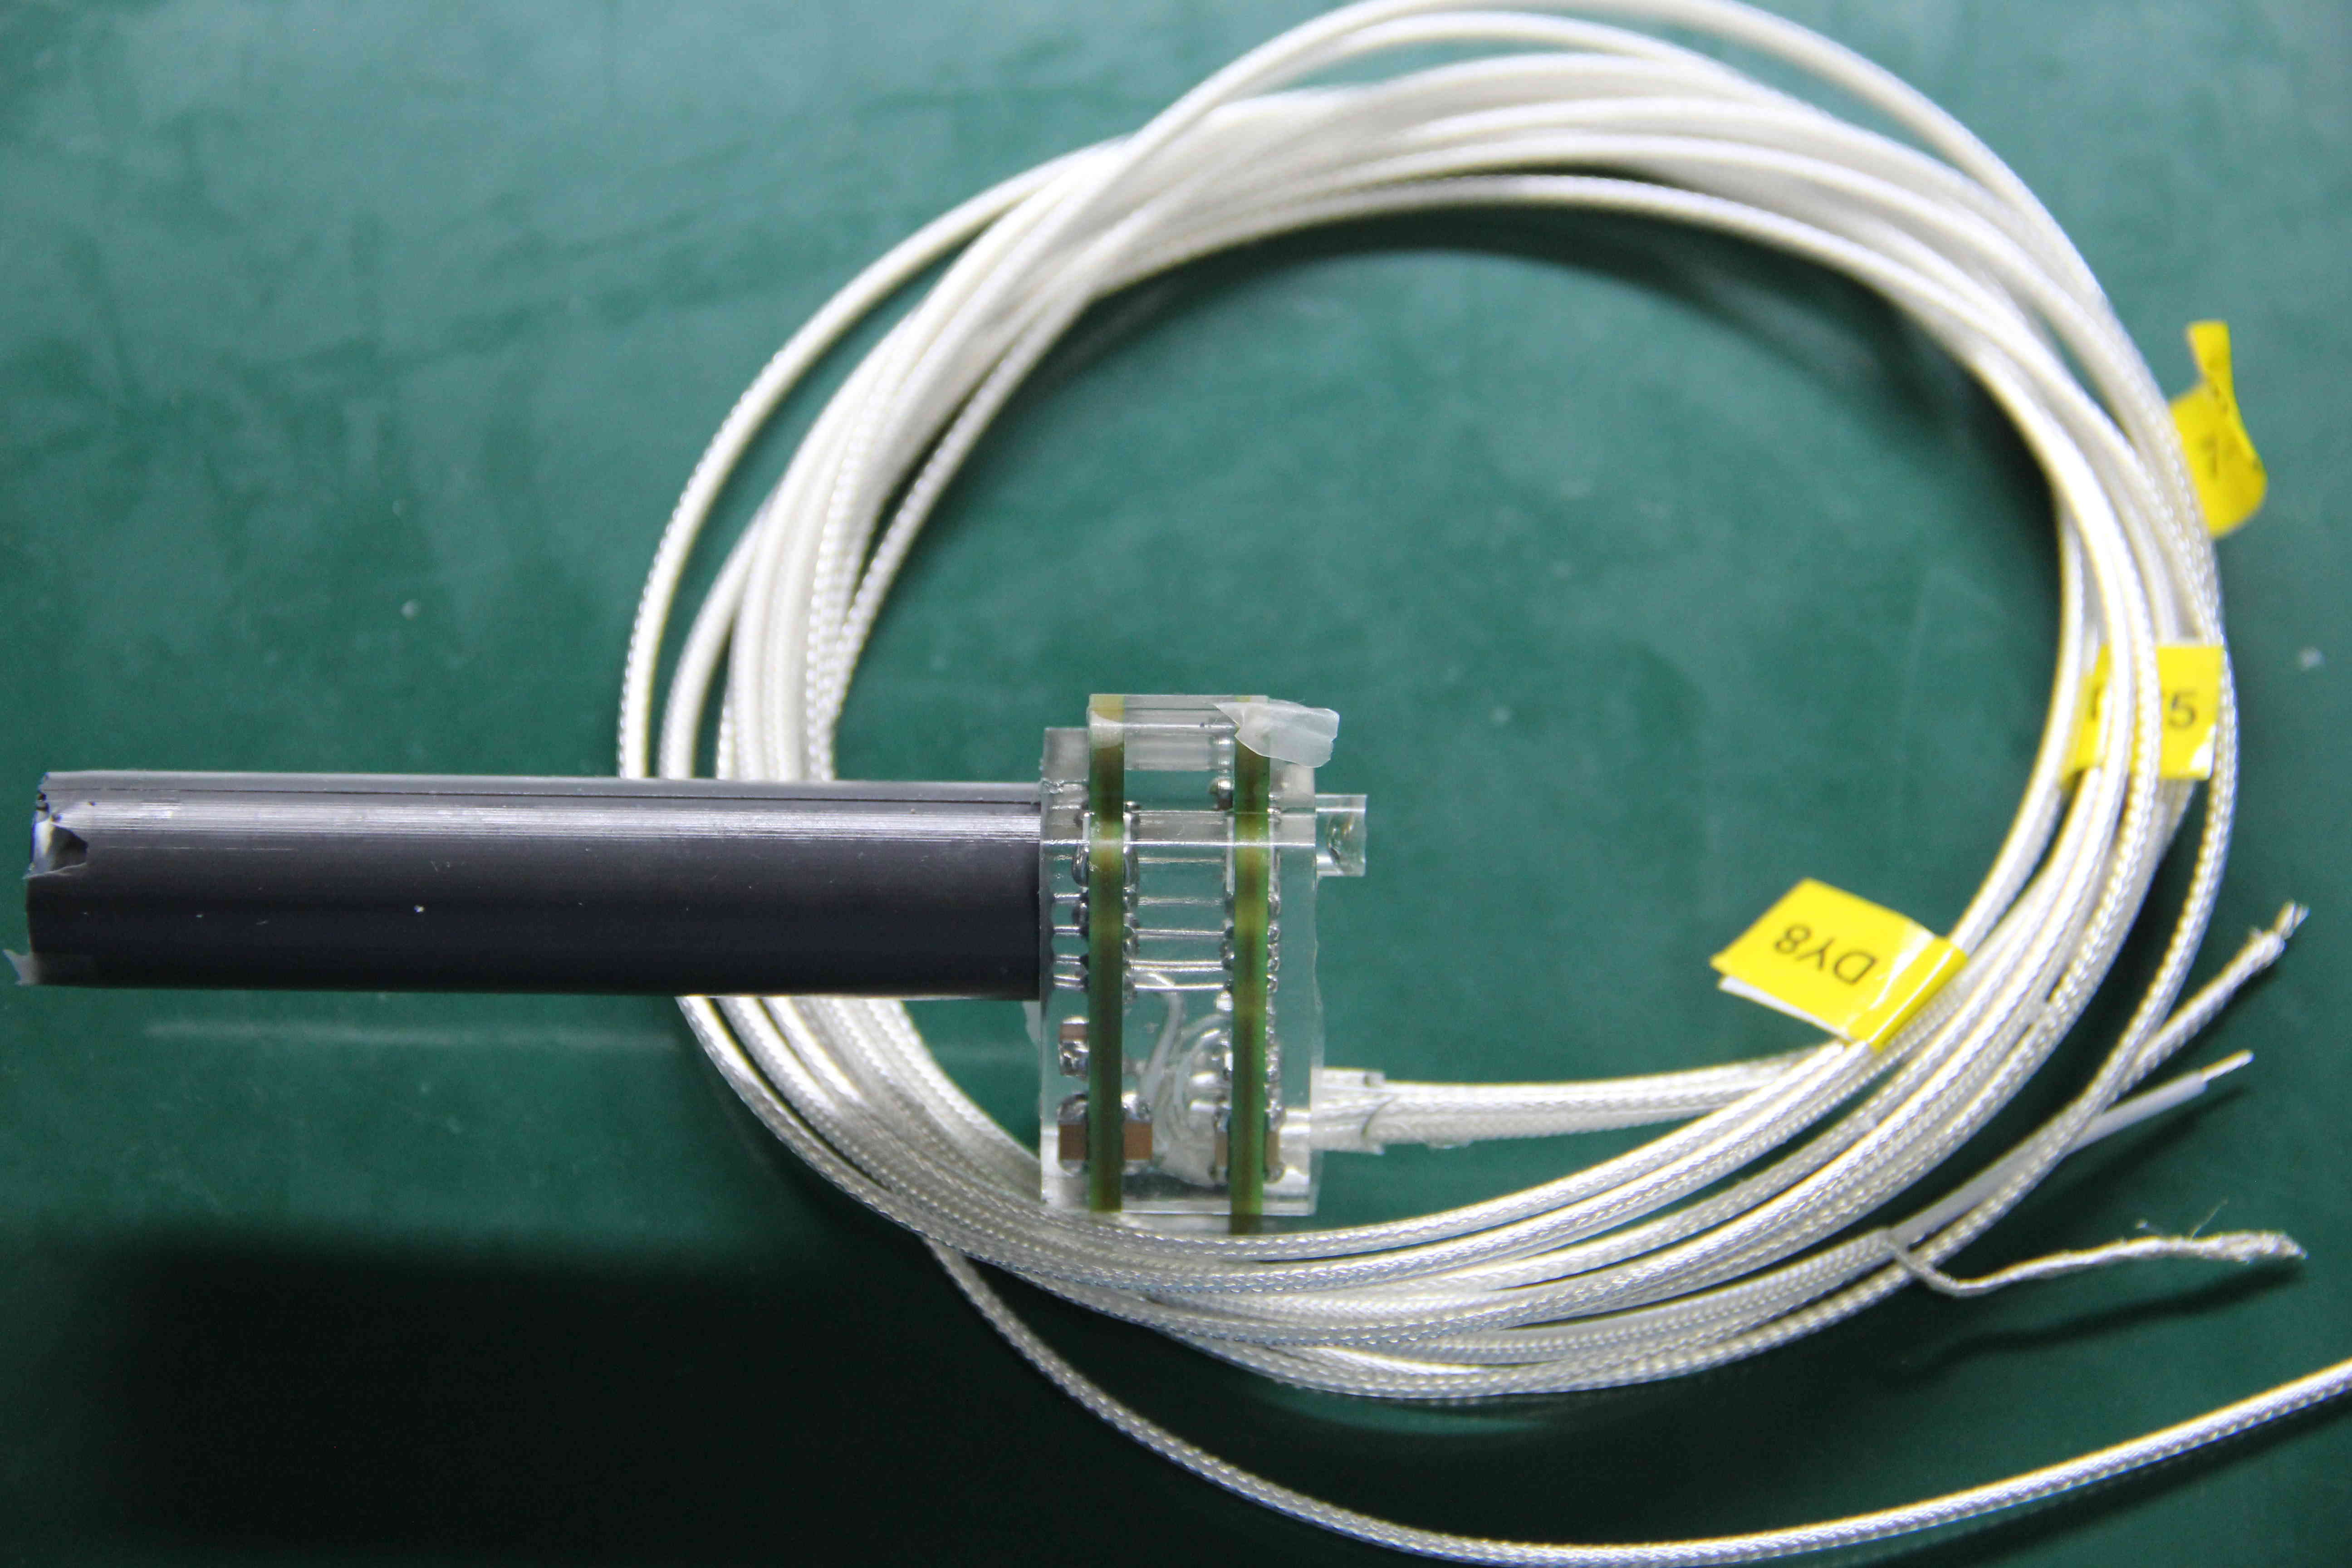
\includegraphics[width=0.65\textwidth]{chap/construction/fig/pmt_assembly.jpg}
	\caption{一个完整的PMT组件}
	\label{fig:construction:pmt_assembly}
\end{figure}

\subsection{生产流程}
\label{sec:construction:pmt_procedure}

\begin{figure}[htbp]
	\centering
	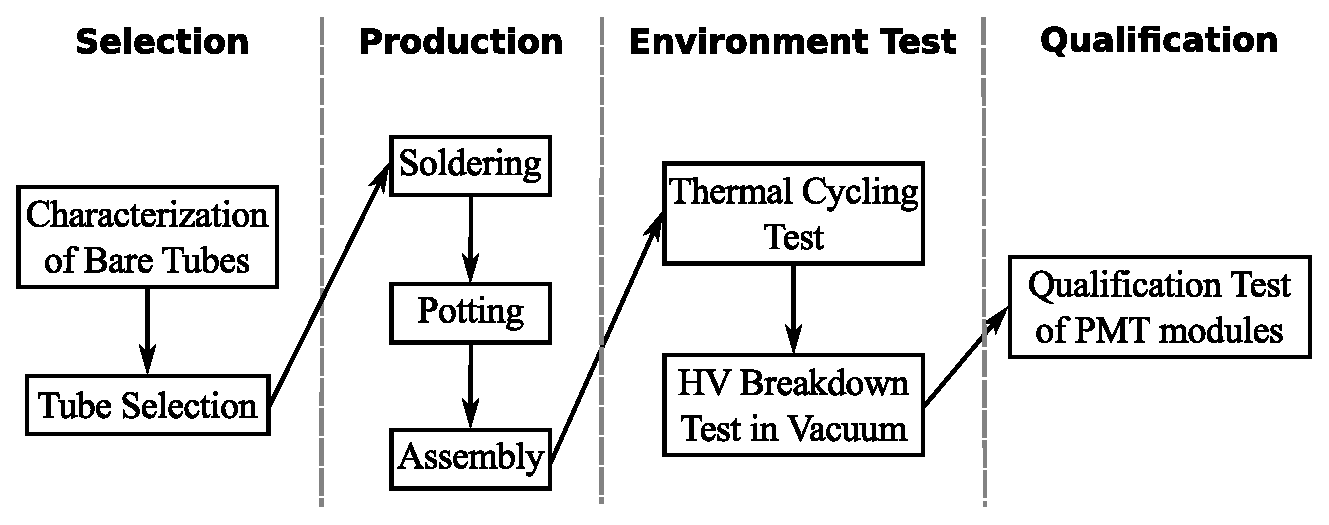
\includegraphics[width=0.95\textwidth]{chap/construction/fig/pmt_production_procedure.eps}
	\caption{PMT组件的生产流程}
	\label{fig:construction:pmt_production_procedure}
\end{figure}

\begin{enumerate}
	\item PMT的base焊接,信号线+信号头。
	\item 检测:电压、电容。
	\item 灌胶。
	\item 高低温循环。
	\item 真空高压测试。
	\item PMT测试平台测试
\end{enumerate}

\section{塑闪单元条的生产}
\label{sec:construction:bar_production}
测试与筛选过程与PMT正好相反,因为单元条需要包装后才能测试。

\subsection{单元条的包装与测试}
\label{sec:construction:bar_wrapping_and_test}

\subsection{单元条的筛选}
\label{sec:construction:bar_selection}
尺寸复核
热膨胀系数
技术衰减长度:平滑否-包装是否好,两端相差较大也踢出,大于一个值
响应均匀性
探测效率
MPV响应?

\section{探测器整体组装}
\label{sec:construction:psd_assembly}

\subsection{PMT与塑闪单元条的匹配}

\begin{enumerate}
	\item 布单元条。
	\item PMT组件加套筒和播磨合金
	\item 上PMT。
	\item 宇宙线测试。
	\item 上高压扇出板
	\item 上FEE盒子(焊接定位用),上FEE转接板
	\item 上高压接头
	\item 正式上FEE盒子
	\item 上FEE电路板
	\item 上顶板
\end{enumerate}
